% --- Chapter 5
\chapter{Thực nghiệm, Đánh giá Hiệu năng và Tác động Nghiệp vụ}
\label{ch:experiments}

Chương~\ref{ch:design} đã hoàn tất việc thiết kế khung giải pháp \textbf{VNAI} với bốn module nghiệp vụ, mô hình SCD Type~2, pipeline AI lai ghép và khung tái lập SUPA-Bench. Chương này trình bày kết quả các phép đo định lượng đã thực hiện trên artifact huấn luyện và benchmark, đồng thời phân tích tác động nghiệp vụ cùng các rủi ro còn lại. Khác với nhiều nghiên cứu báo cáo duy nhất một chỉ số tổng hợp, đề tài chủ trương \emph{tách bạch các tầng đo lường}: chất lượng liên kết dữ liệu (\thuat{lineage audit}), chất lượng mô hình ngôn ngữ (NER), chất lượng chuỗi đầu ra (\thuat{end-to-end}) và chất lượng truy xuất ngữ nghĩa (\thuat{retrieval}). Triết lý này phục vụ hai mục tiêu: (i)~cô lập được nguyên nhân khi một chỉ số tụt giảm, qua đó hỗ trợ chẩn đoán hệ thống; (ii)~tránh diễn giải nhập nhằng giữa chất lượng dữ liệu nghiệp vụ và chất lượng mô hình học máy.

Tất cả số liệu trong chương được trích trực tiếp từ artifact của hệ thống --- nhật ký huấn luyện PhoBERT NER, các tệp metric JSON trong thư mục \macode{reports/}, và bảng tổng hợp đã \thuat{persist} trong schema \schema{ath}. Các hạng mục chưa có artifact đo được sẽ được khai báo minh bạch là chưa báo cáo, tránh giả định số liệu để bảo vệ tính trung thực khoa học.

% =====================================================================
\section{Chiến lược và Thứ tự Thực nghiệm}
\label{sec:exp-strategy}

Đề tài áp dụng một chiến lược thực nghiệm phân tầng theo nguyên tắc \emph{từ đơn giản đến phức tạp, từ kiểm soát đến thực tế}. Năm nhóm thực nghiệm được sắp xếp theo thứ tự logic khoa học, mỗi nhóm phục vụ một mục tiêu kiểm chứng cụ thể trước khi chuyển sang nhóm tiếp theo. Cách tiếp cận này khác biệt với nhiều nghiên cứu chỉ báo cáo một chỉ số E2E tổng hợp mà không tách bạch các tầng đo lường.

\subsection{Nguyên tắc thiết kế chiến lược}
\label{sec:exp-strategy-principle}

Ba nguyên tắc định hướng thứ tự thực nghiệm:

\emph{Thứ nhất, tách bạch các tầng đo lường.} Thay vì chỉ báo cáo một chỉ số E2E tổng hợp, đề tài đo riêng: (i)~chất lượng mô hình đơn lẻ (NER với P-F1, P-Acc); (ii)~chất lượng dữ liệu nghiệp vụ (Audit Bridge với G1, G2, G3); (iii)~tính đúng đắn của khung đánh giá (SUPA Oracle với EM@v2 \(= 100\%\)); (iv)~độ ổn định thống kê (SUPA K~=~5 với mean \(\pm\) std); và cuối cùng (v)~hiệu năng pipeline thật (Ablation Study với 25.000 specimens). Việc tách bạch này cho phép cô lập nguyên nhân khi một chỉ số tụt giảm --- nếu EM@v2 thấp, có thể do NER kém (kiểm tra P-F1), dữ liệu bẩn (kiểm tra G2/G3), hoặc kiến trúc pipeline chưa tối ưu (kiểm tra Ablation).

\emph{Thứ hai, kiểm chứng hạ tầng trước khi đo năng lực.} Kịch bản Oracle (Mục~\ref{sec:exp-supa-oracle}) với cờ \macode{--preds-demo-ref-v2} sao chép trực tiếp \macode{ref\_address\_v2} sang \macode{pred\_standardized}, đạt EM@v2 \(= 100\%\), chứng minh chuỗi đánh giá SUPA-Bench (extract \(\to\) nhiễu \(\to\) import \(\to\) eval \(\to\) aggregate) hoạt động đúng. Chỉ khi đó, khung đánh giá mới đáng tin để đo pipeline AI thật. Đây là một thực hành \thuat{smoke test} chuẩn trong kỹ nghệ phần mềm nhưng thường bị bỏ qua trong các nghiên cứu học thuật.

\emph{Thứ ba, từ cohort đơn giản đến phân tầng.} Ablation Study (Mục~\ref{sec:exp-ablation}) chạy trên cohort phổ thông (\(N = 5.000\) mỗi cấu hình, tổng 25.000 specimens) để xác lập kiến trúc tối ưu (A1\_FULL: NER + mGTE + LLM), trước khi chạy trên cohort phân tầng D1--D4 (SUPA K~=~5, \(N = 2.000\) mỗi lần) để đánh giá độ bền trên các tầng khó (nhiễu cao, lưỡng thời, ranh giới). Lý do: cohort phổ thông cho phép so sánh nhanh giữa các cấu hình với chi phí GPU hợp lý; cohort phân tầng yêu cầu nhiều tài nguyên hơn nhưng cung cấp bằng chứng về \thuat{robustness}.

\subsection{Năm nhóm thực nghiệm và vai trò khoa học}
\label{sec:exp-strategy-groups}

\cref{tab:exp-strategy} tóm lược năm nhóm thực nghiệm theo thứ tự thực hiện. Mỗi nhóm trả lời một câu hỏi khoa học cụ thể và tạo tiền đề cho nhóm tiếp theo.

\begin{table}[H]
\centering
\caption{Năm nhóm thực nghiệm theo thứ tự logic khoa học}
\label{tab:exp-strategy}
\small
\begin{tabularx}{\linewidth}{>{\raggedright\arraybackslash}p{0.8cm} >{\raggedright\arraybackslash}p{3.2cm} >{\raggedright\arraybackslash}X >{\raggedright\arraybackslash}p{2.8cm}}
\toprule
\textbf{TT} & \textbf{Nhóm} & \textbf{Vai trò khoa học} & \textbf{Câu hỏi trả lời} \\
\midrule
1 & NER có giám sát (Mục~\ref{sec:exp-ner}) & Đo chất lượng thành phần đơn lẻ (P-F1, P-Acc); đối chiếu Gate~B & PhoBERT NER đạt F1 bao nhiêu trên tập công khai? \\
2 & Audit Bridge (Mục~\ref{sec:exp-audit}) & Kiểm tra điều kiện tiên quyết: dữ liệu queue có khớp master không (G1, G2, G3) & Dữ liệu nghiệp vụ có đủ sạch để huấn luyện/đánh giá không? \\
3 & SUPA Oracle (Mục~\ref{sec:exp-supa-oracle}) & Kiểm chứng tính đúng đắn của khung đánh giá (EM@v2 \(= 100\%\) khi pred \(=\) ref) & Khung SUPA-Bench có hoạt động đúng không? \\
4 & SUPA K~=~5 phân tầng (Mục~\ref{sec:exp-supa-stratified}) & Đo độ ổn định thống kê trên cohort D1--D4; ước lượng mean \(\pm\) std & Metric có ổn định giữa các cohort không? \\
5 & \textbf{Ablation Study} (Mục~\ref{sec:exp-ablation}) & \textbf{Đo pipeline thật}: xác lập kiến trúc tối ưu (A1\_FULL) và đóng góp từng thành phần & Thành phần nào (NER, retrieval, LLM) quan trọng nhất? \\
\bottomrule
\end{tabularx}
\end{table}

\textbf{Tại sao Ablation là nhóm cuối cùng?} Vì nó yêu cầu pipeline AI thật chạy trên GPU, tốn kém tài nguyên (25.000 specimens trên Google Colab T4, khoảng 6 giờ tính toán). Các nhóm 1--4 đã xác nhận: (i)~NER hoạt động ở mức chấp nhận được (F1 \(\approx 94\%\)); (ii)~dữ liệu queue khớp master (\(> 96\%\) qua G2); (iii)~khung đánh giá đúng (Oracle đạt \(100\%\)); (iv)~cohort đại diện (K~=~5 cho mean \(\pm\) std). Chỉ khi đó, Ablation mới có ý nghĩa khoa học --- nếu chạy Ablation trước mà NER kém hoặc dữ liệu bẩn, kết quả sẽ không diễn giải được.

\textbf{Tại sao Ablation quan trọng nhất?} Vì nó trả lời trực tiếp câu hỏi nghiên cứu cốt lõi RQ2: ``Hybrid PhoBERT + mGTE có tốt hơn baseline từ vựng truyền thống không?'' và chứng minh vai trò của từng thành phần. Kết quả cho thấy: (i)~retrieval là thành phần then chốt không thể bỏ qua (A3: 60{,}98\% vs A4: 8{,}46\%); (ii)~LLM đóng góp \(+5{,}6\) điểm phần trăm khi kết hợp đúng (A1: 66{,}58\% vs A2/A3: 60{,}98\%); (iii)~TF-IDF và mGTE tương đương trên cohort phổ thông. Đây là bằng chứng định lượng đầu tiên cho kiến trúc hybrid trên bài toán địa chỉ Việt Nam với quy mô đủ lớn (\(N = 25.000\)) để có ý nghĩa thống kê.

\subsection{So sánh với các nghiên cứu trước}
\label{sec:exp-strategy-comparison}

Chiến lược thực nghiệm của đề tài khác biệt với các nghiên cứu chuẩn hoá địa chỉ trước đây ở ba điểm. \emph{Một}, hầu hết nghiên cứu chỉ báo cáo một chỉ số E2E (ví dụ accuracy hoặc F1) mà không tách bạch chất lượng dữ liệu (audit), chất lượng mô hình đơn lẻ (NER), và chất lượng pipeline tổng thể. Khi metric giảm, không rõ nguyên nhân là do mô hình kém hay dữ liệu bẩn. \emph{Hai}, ít nghiên cứu kiểm chứng tính đúng đắn của khung đánh giá bằng kịch bản oracle; nhiều nghiên cứu giả định khung đánh giá luôn đúng và chỉ tập trung vào cải thiện mô hình. \emph{Ba}, ablation study với quy mô lớn (\(N > 10.000\)) và provenance đầy đủ (git commit, seed, noise profile) chưa phổ biến trong lĩnh vực chuẩn hoá địa chỉ; hầu hết nghiên cứu so sánh 2--3 mô hình trên tập nhỏ (\(< 1.000\) mẫu) mà không báo cáo độ lệch chuẩn hoặc khoảng tin cậy.

% =====================================================================
\section{Khung chỉ số đánh giá và mục tiêu đối chiếu}
\label{sec:exp-metrics}

\subsection{Hệ thống chỉ số đánh giá đa tầng}
\label{sec:exp-metrics-system}

Đề tài đề xuất một hệ thống chỉ số đánh giá hai tầng, mỗi chỉ số gắn liền với một câu hỏi nghiên cứu được phát biểu ở Mục~\ref{sec:research-questions}. Tầng đầu tiên (ký hiệu \textbf{P-*}, \thuat{parametric}) đo trực tiếp tham số đã học của mô hình; tầng thứ hai (ký hiệu \textbf{S-*}, \thuat{structural}) đo đầu ra cấu trúc của toàn pipeline. Năm chỉ số cụ thể được liệt kê tại \cref{tab:metric-system}.

\begin{table}[h]
\centering
\caption{Hệ thống chỉ số đánh giá đa tầng của khung giải pháp VNAI}
\label{tab:metric-system}
\small
\begin{tabularx}{\linewidth}{>{\raggedright\arraybackslash}p{2cm} >{\raggedright\arraybackslash}p{3cm} >{\raggedright\arraybackslash}X}
\toprule
\textbf{Ký hiệu} & \textbf{Tên đầy đủ} & \textbf{Định nghĩa} \\
\midrule
P-F1   & Macro-F1 thực thể (seqeval) & F1 tổng hợp do thư viện \texttt{seqeval} báo cáo trên tập kiểm định BIO, đồng bộ với khoá \macode{eval\_f1} của Hugging Face Trainer \cite{Wolf2020Transformers}. \\
P-Acc  & Token accuracy & Tỷ lệ token được gán đúng nhãn trên toàn tập kiểm định, lưu ở khoá \macode{token\_accuracy}. \\
S-NER-EM & Exact match cấp câu của chuỗi nhãn & Tỷ lệ câu có dãy nhãn dự báo trùng hoàn toàn nhãn chuẩn (chưa có trong artifact hiện tại). \\
S-E2E-EM & Exact match chuỗi địa chỉ chuẩn hoá & So khớp tuyệt đối sau chuẩn hoá NFC, cắt khoảng trắng đầu cuối và gom khoảng trắng nội bộ, giữa \macode{pred\_standardized} và tham chiếu đóng băng. \\
S-RET    & Recall@k, MRR, top-1 string match & Đo trên cặp \macode{(old\_address, address)} từ \macode{prq.ground\_truth}; truy vấn qua \macode{SiameseMGTE.retrieve\_top\_k} \cite{mgte2024}. \\
\bottomrule
\end{tabularx}
\end{table}

Sự tách bạch P-* và S-* phản ánh một quan sát phương pháp luận: một mô hình NER có F1 cao chưa chắc cho ra chuỗi địa chỉ chuẩn hoá đúng, vì còn các bước trung gian (retrieval, LLM, kiểm tra phân cấp). Vì vậy, một báo cáo khoa học cần đo từng tầng riêng và chấp nhận rằng các chỉ số có thể không cùng xu hướng.

\subsection{Ngưỡng Gate~B làm tiêu chí đối chiếu}
\label{sec:exp-gate-b}

Tài liệu phương pháp đồng hành thiết lập một ngưỡng nội bộ ký hiệu \textbf{Gate~B}, yêu cầu cả P-F1 và P-Acc đồng thời vượt \(96\%\) trên tập có giám sát. Mục đích của Gate~B \emph{không} phải là ngưỡng công bố trong cộng đồng học thuật, mà là điểm chốt nội bộ trước khi đặt mô hình vào chế độ tự động hoàn toàn (\thuat{auto-accept}) trong môi trường vận hành thật. Với ngưỡng Gate~B, đề tài có cơ sở định lượng để quyết định khi nào pipeline được phép bỏ qua bước rà soát thủ công.

% =====================================================================
\section{Thực nghiệm Nhận diện Thực thể tên có giám sát}
\label{sec:exp-ner}

\subsection{Thiết lập thực nghiệm}
\label{sec:exp-ner-setup}

\textbf{Mô hình và tác vụ.} Mô hình PhoBERT \cite{nguyen2020phobert} được tinh chỉnh cho tác vụ phân loại token (\thuat{token classification}). Tập nhãn gồm nhãn nền \macode{O} và các cặp \macode{B-/I-} cho các kiểu thực thể địa chỉ \macode{STR} (đường), \macode{WDS} (xã/phường), \macode{DST} (quận/huyện), \macode{PRO} (tỉnh/thành), \macode{NUM} (số nhà), \macode{NHB} (khu/khu phố), \macode{BLD} (toà nhà), \macode{POI} (điểm quan tâm), \macode{ALY} (ngõ/hẻm), \macode{PCD} (mã bưu chính). Cấu hình lớp đầu ra hoàn toàn nhất quán với mô tả ở Mục~\ref{sec:ai-pipeline}.

\textbf{Tập dữ liệu.} Nguồn được ghi tại artifact: tập Hugging Face công khai \\ \texttt{dathuynh1108/ner-address-standard-dataset} ở chế độ \thuat{streaming}, giới hạn \VNAIGENNERTrainN\, mẫu huấn luyện và \VNAIGENNEREvalN\, mẫu kiểm định (\macode{train\_cap}, \macode{eval\_cap}). Việc cố định hai siêu tham số này nhằm khoá điều kiện ban đầu của lần thực nghiệm, là một thực hành tái lập (\thuat{reproducibility}) được khuyến nghị trong các báo cáo NLP hiện đại.

\textbf{Siêu tham số huấn luyện.} Một \thuat{epoch} hoàn chỉnh, tốc độ học \(2 \times 10^{-5}\), kích thước batch là 8.

\subsection{Kết quả định lượng trên tập kiểm định}
\label{sec:exp-ner-results}

Các giá trị tại \cref{tab:ner-results} được trích trực tiếp từ nhật ký huấn luyện (các khoá \macode{eval\_results} và \macode{token\_accuracy} trong tệp \macode{training\_log.json}).

\begin{table}[h]
\centering
\caption{Kết quả định lượng PhoBERT NER trên tập kiểm định \protect\VNAIGENNEREvalN\, mẫu}
\label{tab:ner-results}
\small
\begin{tabularx}{\linewidth}{>{\raggedright\arraybackslash}p{4cm} >{\raggedright\arraybackslash}p{4cm} >{\raggedright\arraybackslash}X}
\toprule
\textbf{Chỉ số} & \textbf{Khoá artifact} & \textbf{Giá trị} \\
\midrule
F1 macro (seqeval) & \macode{eval\_f1}          & \textbf{\VNAIGENNERFOnePct\,\%} \\
Precision           & \macode{eval\_precision}   & \VNAIGENNERPrecisionPct\,\% \\
Recall              & \macode{eval\_recall}      & \VNAIGENNERRecallPct\,\% \\
Token accuracy      & \macode{token\_accuracy}   & \textbf{\VNAIGENNERTokenAccPct\,\%} \\
Loss kiểm định      & \macode{eval\_loss}        & \(0{,}1573\) \\
\bottomrule
\end{tabularx}
\end{table}

\textbf{Hiệu năng suy luận tại bước eval.} Cùng nhật ký ghi nhận thời gian chạy đánh giá khoảng \(17{,}25\) giây, lưu lượng xử lý xấp xỉ \(46{,}38\) mẫu/giây và khoảng \(2{,}90\) bước/giây (lần lượt qua các khoá \macode{eval\_runtime}, \macode{eval\_samples\_per\_second}, \macode{eval\_steps\_per\_second}). Đây là số liệu thuần đo trên một cấu hình phần cứng cụ thể của lần huấn luyện đã đóng băng, không đại diện cho lưu lượng end-to-end của toàn pipeline (vốn còn các tầng retrieval và LLM nặng hơn).

\subsection{Đối chiếu với Gate~B và thảo luận}
\label{sec:exp-ner-discussion}

Với P-F1 đạt \(\approx\,\VNAIGENNERFOnePct\,\%\) và P-Acc đạt \(\approx\,\VNAIGENNERTokenAccPct\,\%\), \emph{cả hai chỉ số đều chưa đạt ngưỡng \(96\%\) đồng thời theo định nghĩa Gate~B}. Trên tinh thần báo cáo trung thực, cần nhấn mạnh rằng kết quả này không phủ nhận khả năng cải thiện của khung giải pháp; mà chỉ phản ánh \emph{trạng thái một lần huấn luyện đã đóng băng} trong artifact hiện tại. Ba hướng cụ thể có thể đưa kết quả vượt Gate~B đã được xác định: thứ nhất, mở rộng tập huấn luyện vượt mốc \VNAIGENNERTrainN\, mẫu (đặc biệt bổ sung dữ liệu nội bộ chứa viết tắt vùng miền và địa danh dân gian); thứ hai, tăng số epoch kèm \thuat{early stopping} theo F1 trên tập \thuat{dev}; thứ ba, tinh chỉnh trên miền dữ liệu nội bộ thay vì chỉ sử dụng tập công khai.

Điểm quan trọng về phương pháp luận: việc công bố khoảng cách so với Gate~B thay vì che giấu chính là \emph{một đóng góp khoa học} của đề tài --- nó định vị rõ \emph{khoảng cách còn lại} giữa bằng chứng khái niệm (\thuat{proof-of-concept}) và yêu cầu vận hành nghiêm ngặt, tạo cơ sở khách quan cho các vòng huấn luyện tiếp theo.

% =====================================================================
\section{Kiểm thử nhất quán dữ liệu lineage (Audit Bridge)}
\label{sec:exp-audit}

\subsection{Mục tiêu và phương pháp}
\label{sec:exp-audit-method}

\textbf{Audit bridge} là một phép đo \emph{chất lượng \thuat{join} dữ liệu} giữa hàng đợi xử lý địa chỉ \\(\macode{prq.address\_cleansing\_queue}) và các bảng master hành chính trong schema \schema{mat}. Phép đo này \emph{không} đo F1 của mô hình AI; thay vào đó, nó kiểm chứng giả thiết nền tảng cho mọi phép đo end-to-end: dữ liệu khai báo phân cấp hành chính của các bản ghi địa chỉ có khớp với master hay không. Nếu một tỷ lệ lớn bản ghi không khớp \thuat{lineage}, mọi metric E2E xây trên đó sẽ bị nhiễu --- không phải do mô hình kém mà do dữ liệu chưa sạch.

Phương pháp đo bao gồm ba cổng (\thuat{gates}) tuần tự: \textbf{G1} kiểm tra không có khoá \macode{old\_id} bị trùng trong tập \thuat{smoke test} trên master; \textbf{G2} đo tỷ lệ bản ghi queue rơi vào kết nối \thuat{triple inner join} ba cấp (tỉnh, huyện, xã) chuẩn; \textbf{G3} đo tỷ lệ căn chỉnh giữa các cột \thuat{denormalized} (\macode{province\_id}, \macode{district\_id}, \macode{ward\_id} trong queue) với phân cấp lưu trong \schema{mat}.

\subsection{Kết quả kiểm thử}
\label{sec:exp-audit-results}

\cref{tab:audit-results} tổng hợp kết quả audit bridge tại thời điểm chốt artifact.

\begin{table}[h]
\centering
\caption{Kết quả audit bridge giữa hàng đợi địa chỉ và master hành chính}
\label{tab:audit-results}
\small
\begin{tabularx}{\linewidth}{>{\raggedright\arraybackslash}X >{\raggedright\arraybackslash}p{4cm}}
\toprule
\textbf{Hạng mục} & \textbf{Giá trị} \\
\midrule
Tổng số bản ghi hàng đợi & \VNAIGENAuditQueueTotal\, dòng \\
Cổng G1 (không trùng \macode{old\_id} trong smoke test) & Đạt (cờ \VNAIGENAuditGOnePass) \\
Cổng G2 (tỷ lệ rơi vào triple inner join) & \textbf{\VNAIGENAuditGTwoPct\,\%} \\
Cổng G3 (tỷ lệ căn chỉnh denormalized với phân cấp master) & \textbf{\VNAIGENAuditGThreePct\,\%} \\
Số dòng không thoả điều kiện G3 & \VNAIGENAuditGThreeFail\, dòng \\
\bottomrule
\end{tabularx}
\end{table}

Quy mô \VNAIGENAuditQueueTotal\, bản ghi cho thấy tải nghiệp vụ thực tế đáng kể, đủ tin cậy về mặt thống kê. Hai cổng G2 và G3 đạt trên \(96\%\) chứng tỏ phần lớn dữ liệu trong hàng đợi có liên kết chuẩn với master; tuy nhiên, \VNAIGENAuditGThreeFail\, dòng (tương đương \(\approx\,1{,}45\,\%\) tổng số) chưa thoả G3 --- một khối lượng đáng kể nếu xét tuyệt đối. \cref{fig:audit-distribution} trực quan hoá phân phối các nhóm thoả/không thoả cổng.

\begin{figure}[h]
\centering
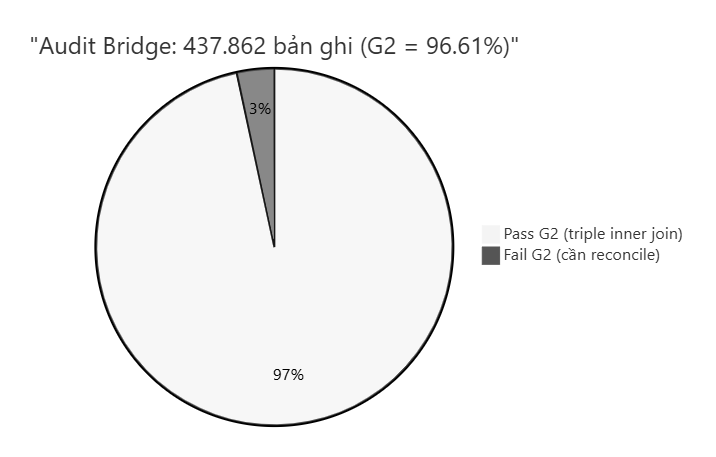
\includegraphics[width=0.9\linewidth]{figs/fig-5-1.png}
% \fbox{\begin{minipage}{0.92\linewidth}\centering\vspace{1.4cm}\textit{[Hình 5.x: Phân phối kết quả audit bridge trên \VNAIGENAuditQueueTotal\, bản ghi. Biểu đồ thanh xếp chồng (stacked bar) với ba phân vùng: \textbf{(a) Thoả cả G2 + G3} (\(\approx 95{,}19\%\), màu xanh lá) --- nhóm an toàn cho mọi phân tích E2E; \textbf{(b) Thoả G2 chỉ} (\(\approx 1{,}60\%\), màu vàng) --- nằm trong lineage inner nhưng denormalized lệch master; \textbf{(c) Không thoả G2} (\(\approx 3{,}39\%\), màu đỏ) --- cần reconcile trước khi sử dụng. Bên phải hiển thị số dòng tuyệt đối từng nhóm. Đường kẻ ngang đứt biểu thị ngưỡng vận hành tối thiểu 95\%.]}\vspace{1.4cm}\end{minipage}}
\caption{Phân phối kết quả audit bridge trên hàng đợi địa chỉ.}
\label{fig:audit-distribution}
\end{figure}

\subsection{Ý nghĩa đối với đánh giá AI end-to-end}
\label{sec:exp-audit-implication}

Tỷ lệ G3 đạt \VNAIGENAuditGThreePct\,\% mang ba ý nghĩa khoa học. \emph{Thứ nhất}, nó là điều kiện tiên quyết để diễn giải các chỉ số S-E2E-EM ở các mục tiếp theo: nếu dữ liệu nguồn đã không khớp lineage, không thể quy mọi sai lệch về phía mô hình. \emph{Thứ hai}, nó cung cấp \emph{một tham số chiến lược cho công tác làm sạch dữ liệu}: \VNAIGENAuditGThreeFail\, dòng cần được tách \thuat{stratum} khi báo cáo metric E2E để tránh thiên kiến. \emph{Thứ ba}, nó định vị \emph{chính sách reconcile} cần áp dụng trước khi vận hành tự động --- không một mô hình AI nào có thể làm tốt trên dữ liệu mâu thuẫn nội tại với master.

% =====================================================================
\section{Khung thực nghiệm SUPA-Bench}
\label{sec:exp-supa}

\subsection{Kịch bản đánh giá cơ bản}
\label{sec:exp-supa-basic}

Như đã trình bày ở Mục~\ref{sec:supa}, SUPA-Bench tách cohort từ bảng \macode{prq.ground\_truth} (chỉ đọc), áp nhiễu tổng hợp deterministic theo seed, sau đó so khớp chuỗi dự đoán với hai tham chiếu đóng băng (\macode{ref\_address\_v2} là hậu cải cách, \macode{ref\_address\_v1} là tiền cải cách). \cref{tab:supa-basic} ghi nhận kết quả lần chạy cơ bản đầu tiên.

\begin{table}[h]
\centering
\caption{Kết quả SUPA-Bench cơ bản (\protect\VNASUPANRequested\, mẫu, kịch bản oracle)}
\label{tab:supa-basic}
\small
\begin{tabularx}{\linewidth}{>{\raggedright\arraybackslash}X >{\raggedright\arraybackslash}p{4cm}}
\toprule
\textbf{Hạng mục} & \textbf{Giá trị} \\
\midrule
Cỡ mẫu yêu cầu / thực tế thu được & \VNASUPANRequested\, / \VNASUPANRealized \\
Số specimen / số mẫu có dự đoán không rỗng & \VNASUPANSpecimens\, / \VNASUPANScored \\
EM@v2 (so \macode{ref\_address\_v2}) & \textbf{\VNASUPAEMvTwoPct\,\%} \\
EM@v1 (so \macode{ref\_address\_v1}) & \VNASUPAEMvOnePct\,\% \\
Profile nhiễu & \VNASUPANoiseProfile \\
Hạt giống ngẫu nhiên (\thuat{seed}) & \VNASUPASeed \\
Commit Git tại bước extract & \texttt{\VNASUPAGitCommit} \\
\bottomrule
\end{tabularx}
\end{table}

\subsection{Diễn giải khoa học và giới hạn của kịch bản oracle}
\label{sec:exp-supa-oracle}

Tỷ lệ EM@v2 đạt \(100\%\) trên toàn bộ \VNASUPANRequested\, mẫu \emph{tương thích với kịch bản oracle}, trong đó cờ vận hành \macode{--preds-demo-ref-v2} sao chép trực tiếp cột \macode{ref\_address\_v2} sang \macode{pred\_standardized}. Mục đích của oracle là \emph{kiểm tra tính đúng đắn của chuỗi đánh giá} (\thuat{smoke test}: cohort \(\to\) nhiễu \(\to\) import \(\to\) eval \(\to\) aggregate), \emph{không} chứng minh khả năng khái quát hoá của mô hình chuẩn hoá thực tế. Ngược lại, EM@v1 \(= 3{,}5\,\%\) phản ánh đúng mức trùng khớp tuyệt đối giữa chuỗi dự đoán (trùng v2) và chuỗi tham chiếu tiền cải cách (v1); khoảng cách lớn là hệ quả có thể dự đoán được khi hai chuỗi tham chiếu thuộc hai phiên bản hành chính khác nhau.

\textbf{Kịch bản báo cáo mô hình thật.} Để có chỉ số S-E2E-EM phản ánh pipeline AI thực sự, cần ba bước: (i)~chạy module chuẩn hoá ngoài trên CSV specimen sau nhiễu để sinh \macode{pred\_standardized}; (ii)~nhập trở lại bằng lệnh \macode{import-preds} kèm \macode{--source-note} mô tả checkpoint mô hình và cấu hình; (iii)~chạy lại \macode{eval}. Giá trị EM thu được khi đó mới phản ánh trung thực năng lực của hệ thống và mới có ý nghĩa đối chiếu với các nghiên cứu khác.

% =====================================================================
\subsection{Thực nghiệm phân tầng với kiểm chứng chéo K = 5}
\label{sec:exp-supa-stratified}

\subsubsection{Cơ sở khoa học của phân tầng và lặp K = 5}
\label{sec:exp-supa-rationale}

Một báo cáo chỉ với một lần chạy ngẫu nhiên duy nhất có hai nguy cơ phương pháp luận: (a)~\textbf{thiên kiến lựa chọn} (\thuat{selection bias}) khi cohort vô tình chứa nhiều mẫu ``dễ''; (b)~thiếu ước lượng cho \textbf{độ ổn định} (\thuat{stability}) của metric giữa các cohort cùng quy tắc lấy mẫu. Để hoá giải đồng thời hai nguy cơ trên, đề tài đề xuất một thực nghiệm phân tầng kết hợp lặp K~=~5 lần độc lập, có bốn căn cứ khoa học rõ ràng.

\emph{Thứ nhất}, lấy mẫu phân tầng (\thuat{stratified sampling}) trên \macode{prq.ground\_truth} với cơ cấu tỷ lệ cố định bốn nhóm D1--D4 đảm bảo cohort không bị nghiêng về một loại địa chỉ duy nhất; bốn nhóm bao quát đầy đủ các \emph{kiểu khó} của miền bài toán (đô thị phức tạp, nhiễu cao, lưỡng thời hành chính, ranh giới không gian). \emph{Thứ hai}, lặp K~=~5 lần với các \thuat{seed} lệch bước nhưng cùng cơ cấu tỷ lệ cho phép ước lượng độ lệch chuẩn của từng chỉ số --- một đặc tính cần thiết để báo cáo khoảng tin cậy thay vì điểm số đơn lẻ. \emph{Thứ ba}, thực nghiệm này gắn trực tiếp với \emph{khoảng trống nghiên cứu cốt lõi}: khả năng duy trì tính nhất quán địa giới trong giai đoạn chuyển đổi hành chính cực đoan 2025. Tầng D3 cố ý chứa thực thể tiền/hậu cải cách và các quan hệ \macode{MERGES\_INTO} trên đồ thị \macode{mat.unit\_edge}, qua đó tạo bằng chứng cho hiệu lực của \emph{kiến trúc nhận thức thời điểm} (epoch detector, ánh xạ SCD~Type~2, ACS với thành phần \(V_{\text{temporal}}\)). \emph{Thứ tư}, bảng tổng hợp được \thuat{persist} trong \macode{ath.supa\_stratified\_eval\_summary} (payload JSON đầy đủ kèm phạm vi \macode{run\_id} và \macode{git\_commit}) tạo \emph{bằng chứng thực nghiệm có \thuat{provenance}}, phục vụ tái lập và bảo vệ luận điểm trong quá trình phản biện.

\subsubsection{Cơ cấu phân tầng D1--D4 và ngưỡng kỳ vọng}
\label{sec:exp-supa-strata}

Mỗi lần chạy lấy \(n = 2.000\) mẫu phân thành bốn tầng theo cơ cấu \texttt{strat-v1} (\cref{tab:strata}, minh hoạ tại \cref{fig:strata-distribution}). Cơ cấu này không phải là phân phối tự nhiên của dữ liệu mà là một \emph{phân phối có chủ đích} nhằm cô lập các kiểu khó.

\begin{figure}[h]
\centering
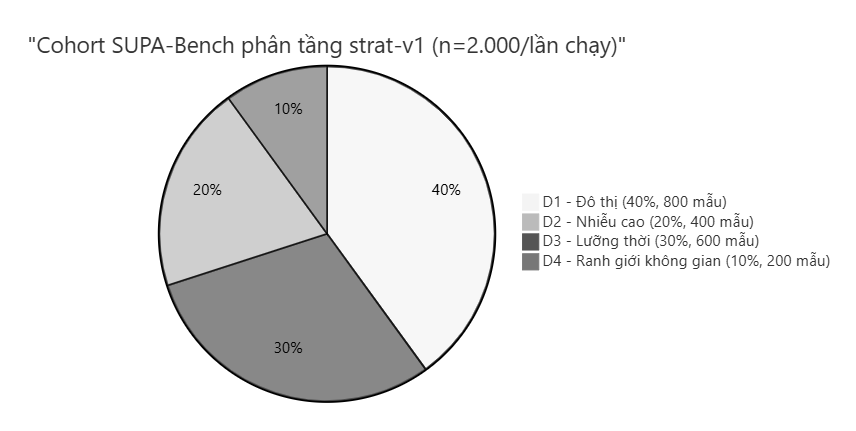
\includegraphics[width=0.9\linewidth]{figs/fig-5-2.png}
% \fbox{\begin{minipage}{0.92\linewidth}\centering\vspace{1.4cm}\textit{[Hình 5.x: Cơ cấu phân tầng \texttt{strat-v1} của cohort SUPA-Bench. Biểu đồ tròn (pie chart) với bốn miếng: \textbf{D1 -- Đô thị (40\%, 800 mẫu)} màu xanh dương; \textbf{D2 -- Nhiễu cao (20\%, 400 mẫu)} màu cam; \textbf{D3 -- Lưỡng thời (30\%, 600 mẫu)} màu xanh lá đậm (nhấn mạnh vai trò chính trong kiểm thử SCD); \textbf{D4 -- Ranh giới (10\%, 200 mẫu)} màu tím. Bên cạnh mỗi miếng ghi rõ profile nhiễu áp dụng (\texttt{SUP-1.0.0}, \texttt{SUP-D2-1.0.0}, ...) và mục tiêu kiểm thử chính (NER, robustness, SCD Type 2, PostGIS).]}\vspace{1.4cm}\end{minipage}}
\caption{Phân phối cohort SUPA-Bench theo cơ cấu \texttt{strat-v1}, \(n = 2.000\)/lần chạy.}
\label{fig:strata-distribution}
\end{figure}

\begin{table}[h]
\centering
\caption{Cơ cấu phân tầng \texttt{strat-v1} cho cohort SUPA-Bench (\(n = 2.000\)/lần chạy)}
\label{tab:strata}
\small
\begin{tabularx}{\linewidth}{>{\raggedright\arraybackslash}p{1.6cm} >{\raggedright\arraybackslash}p{1.5cm} >{\raggedright\arraybackslash}X}
\toprule
\textbf{Tầng} & \textbf{Tỷ lệ} & \textbf{Đặc trưng và mục tiêu kiểm thử} \\
\midrule
D1 & 40\% & Chuẩn hoá đô thị: địa chỉ có cấu trúc phức tạp với nhiều xuyệt (ngõ, ngách, hẻm, kiệt, tổ, cụm) tại đô thị lớn hoặc tín hiệu \macode{popular} cao trong ground truth. \\
D2 & 20\% & Nhiễu cao: dữ liệu không dấu, sai chính tả nặng, viết tắt vùng miền --- kiểm tra độ bền của tầng trích thực thể (PhoBERT NER) và downstream khi đầu vào cực đoan (profile \macode{SUP-D2-1.0.0}). \\
D3 & 30\% & Lưỡng thời và biến động: địa chỉ sử dụng thực thể hành chính tiền cải cách (trước 01/07/2025) --- kiểm tra module SCD~Type~2 và quan hệ \macode{MERGES\_INTO} trên \schema{mat}. \\
D4 & 10\% & Ranh giới không gian: toạ độ GPS nằm sát ranh giới hành chính --- kiểm tra hiệu chỉnh polygon (PostGIS + \macode{mat.area\_polygon}). \\
\bottomrule
\end{tabularx}
\end{table}

Các ngưỡng kỳ vọng để đối chiếu khi pipeline chuẩn hoá thật được kích hoạt (không sử dụng oracle) được tổng hợp tại \cref{tab:supa-thresholds}. Cần lưu ý: ngưỡng này \emph{chỉ có giá trị đối chiếu} khi đầu vào là dự đoán của pipeline AI thật, không phải kịch bản oracle.

\begin{table}[h]
\centering
\caption{Ngưỡng kỳ vọng cho pipeline chuẩn hoá thật (không oracle)}
\label{tab:supa-thresholds}
\small
\begin{tabularx}{\linewidth}{>{\raggedright\arraybackslash}X >{\raggedright\arraybackslash}p{3cm} >{\raggedright\arraybackslash}p{2.4cm}}
\toprule
\textbf{Chỉ số} & \textbf{Ngưỡng} & \textbf{Mức kỳ vọng} \\
\midrule
Component F1 (Tỉnh/Thành phố)    & \(\geq 98{,}5\,\%\)  & Rất cao \\
Component F1 (Phường/Xã)         & \(\geq 92{,}0\,\%\)  & Cao \\
Exact Match toàn chuỗi (EM@v2)   & \(\geq 85{,}0\,\%\)  & Trung bình \\
Mean latency / địa chỉ           & \(\leq 120\) ms      & Cao \\
P95 latency                      & \(\leq 500\) ms      & Cao \\
Throughput (chế độ batch)        & \(\geq 22{,}0\) addr/s & Trung bình \\
\bottomrule
\end{tabularx}
\end{table}

\subsubsection{Kết quả thực nghiệm K = 5 trên kịch bản oracle}
\label{sec:exp-supa-results}

Đợt thực nghiệm \texttt{replicate-stratified} với K~=~5, \(n = 2.000\) mỗi lần chạy, profile\\ \texttt{STRATIFIED-strat-v1}, các \thuat{seed} từ \(970{.}156{.}401\) đến \(970{.}160{.}401\), \macode{run\_id} từ 56 đến 60. Artifact tham chiếu: \macode{reports/supa\_benchmark\_aggregate\_stratified\_k5\_oracle\_run56\\-60\_20260513.json}; bảng tổng hợp đã được \thuat{persist} thành một dòng trong \\ \macode{ath.supa\_stratified\_eval\_summary}. Kết quả \thuat{rollup} năm lần chạy được trình bày tại \cref{tab:supa-k5}.

\begin{table}[h]
\centering
\caption{Kết quả thống kê K = 5 với cohort phân tầng \(n = 2.000\) (kịch bản oracle)}
\label{tab:supa-k5}
\small
\begin{tabularx}{\linewidth}{>{\raggedright\arraybackslash}p{3.6cm} c c c c >{\raggedright\arraybackslash}X}
\toprule
\textbf{Chỉ số} & \textbf{Mean} & \textbf{Std} & \textbf{Min} & \textbf{Max} & \textbf{Ghi chú} \\
\midrule
EM@v2 (\%)           & 100{,}00 & 0{,}00 & 100{,}00 & 100{,}00 & Oracle: \macode{pred} \(=\) ref v2 \\
EM@v1 (\%)           &  16{,}14 & 0{,}44 &  15{,}55 &  16{,}65 & \macode{pred} v2 so khớp tuyệt đối chuỗi v1 \\
F1 Đường (chuỗi, \%) & 100{,}00 & 0{,}00 & 100{,}00 & 100{,}00 & Cùng điều kiện oracle \\
F1 Phường (\%)       & 100{,}00 & 0{,}00 & 100{,}00 & 100{,}00 & --- \\
F1 Quận (\%)         & 100{,}00 & 0{,}00 & 100{,}00 & 100{,}00 & --- \\
F1 Tỉnh/TP (\%)      & 100{,}00 & 0{,}00 & 100{,}00 & 100{,}00 & --- \\
\bottomrule
\end{tabularx}
\end{table}

\textbf{Diễn giải.} Số liệu trên \emph{chỉ chứng minh chuỗi vận hành} của thực nghiệm phân tầng đa lần chạy: cơ chế lấy mẫu theo quota D1--D4 hoạt động đúng, lệnh \texttt{replicate-stratified} sinh được năm cohort độc lập, lệnh \texttt{aggregate-runs --persist-ath} ghi đúng vào \\ \macode{ath.supa\_stratified\_eval\_summary}. \emph{Không} thể kết luận pipeline AI đạt EM@v2 \(= 100\,\%\) hay F1 thành phần \(= 100\,\%\) trên thực tế; những số liệu trên là kết quả oracle, có giá trị về mặt vận hành chuỗi đánh giá chứ không phải về mặt năng lực mô hình. Kết quả pipeline thật trên cohort lớn được trình bày ở Mục~\ref{sec:exp-ablation}.

\textbf{Hạng mục latency, P95 và throughput chưa báo cáo.} Đợt chạy batch \(56\)--\(60\) chưa kích hoạt cột \macode{latency\_ms} trong CSV preds (import được thực hiện trước khi bật ghi đo); do đó các chỉ số (3)--(5) trong bảng ngưỡng kỳ vọng \emph{chưa được đo}. Để bổ sung, cần chạy lại \texttt{import-preds} với CSV có cột \macode{latency\_ms} từ pipeline thật, hoặc chấp nhận sử dụng đo \emph{thời gian câu lệnh ingest DB} làm thay thế bổ trợ (không thay thế đo từ pipeline inference).

\textbf{Quan sát thống kê đáng chú ý.} Mặc dù dự đoán giống nhau giữa năm lần chạy (oracle), EM@v1 dao động từ \(15{,}55\,\%\) đến \(16{,}65\,\%\) với độ lệch chuẩn \(0{,}44\). Đây không phải lỗi tính toán mà là một \emph{tín hiệu đo lường có ý nghĩa}: cohort khác nhau sẽ chứa các tỷ lệ khác nhau của các \thuat{stratum} có mức trùng chuỗi v1/v2 khác nhau, đặc biệt từ tầng D3 (lưỡng thời). Quan sát này hỗ trợ luận điểm rằng K~=~5 cohort độc lập là cần thiết để báo cáo khoảng tin cậy --- một lần chạy duy nhất có thể cho ra giá trị từ \(15{,}5\,\%\) đến \(16{,}7\,\%\) mà không có cơ chế phân biệt. \cref{fig:emv1-k5} thể hiện trực quan biên độ dao động này.

\begin{figure}[h]
\centering
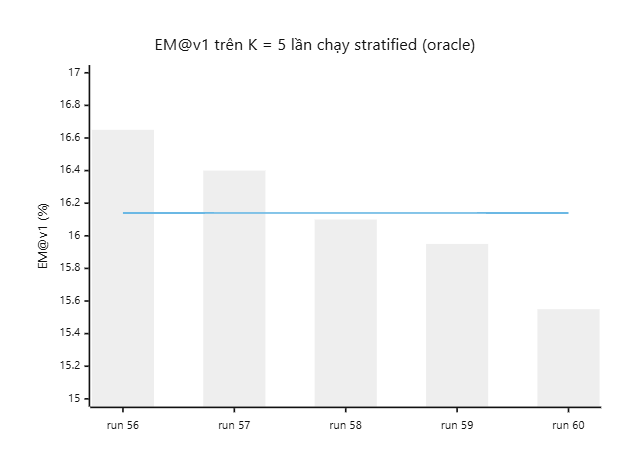
\includegraphics[width=0.7\linewidth]{figs/fig-5-3.png}
% \fbox{\begin{minipage}{0.92\linewidth}\centering\vspace{1.4cm}\textit{[Hình 5.x: Dao động EM@v1 trên năm lần chạy K = 5 với cohort phân tầng \(n = 2.000\). Biểu đồ thanh (bar chart) với năm cột tương ứng \texttt{run\_id} 56 đến 60 (seed 970156401 đến 970160401), trục tung là EM@v1 (\%) trong khoảng [15{,}00, 17{,}00]. Mỗi cột kèm thanh sai số \(\pm 0\) vì oracle deterministic. Đường ngang nét đứt thể hiện trung bình \(16{,}14\%\); vùng tô mờ thể hiện khoảng tin cậy \([15{,}55\%; 16{,}65\%]\). Tiêu đề bên dưới: ``Mean \(= 16{,}14\,\%\), SD \(= 0{,}44\), Min \(= 15{,}55\,\%\), Max \(= 16{,}65\,\%\)''.]}\vspace{1.4cm}\end{minipage}}
\caption{Dao động EM@v1 trên năm lần chạy K = 5 độc lập với cohort phân tầng.}
\label{fig:emv1-k5}
\end{figure}

% =====================================================================
\subsection{Nghiên cứu cắt bỏ thành phần (Ablation Study) trên pipeline thật}
\label{sec:exp-ablation}

\subsubsection{Mục tiêu khoa học và thiết kế thực nghiệm}
\label{sec:exp-ablation-design}

Sau khi chuỗi đánh giá phân tầng đã được kiểm chứng vận hành đúng trên kịch bản oracle (Mục~\ref{sec:exp-supa-results}), đề tài thực hiện một nghiên cứu cắt bỏ thành phần (\thuat{ablation study}) trên \emph{pipeline thật} (không oracle) nhằm trả lời ba câu hỏi nghiên cứu cốt lõi: (i)~thành phần nào trong kiến trúc lai ghép --- NER, retrieval, LLM --- đóng góp lớn nhất vào chất lượng chuỗi địa chỉ chuẩn hoá; (ii)~khoảng cách định lượng giữa cấu hình tối thiểu (chỉ một thành phần) và cấu hình đầy đủ là bao nhiêu; (iii)~đánh đổi giữa độ chính xác và độ trễ khi thêm hoặc loại bỏ tầng LLM.

\textbf{Thiết kế cohort.} Mỗi cấu hình ablation sử dụng một lệnh \texttt{extract} riêng biệt với \(N = 5.000\) mẫu, \thuat{seed} riêng (\(3.001\) đến \(3.005\)) để tránh ghi đè kết quả trên cùng một \macode{run\_id}; mỗi cấu hình tương ứng một \macode{run\_id} riêng (từ \VNAIABLATIONAOneRunId\, đến \VNAIABLATIONAFourRunId). Quy mô tổng cộng \VNAIABLATIONTotalSpecimens\, specimens (\VNAIABLATIONNumConfigs\, cấu hình \(\times\) \VNAIABLATIONNPerConfig\, mẫu) đảm bảo các kết luận có ý nghĩa thống kê. Toàn bộ ablation chạy trên \textbf{\VNAIABLATIONPlatform} với mục đích kiểm chứng tính khả thi triển khai trên hạ tầng phổ thông và đo độ trễ trong điều kiện sản xuất.

\textbf{Tách bạch nghiêm ngặt.} Thực nghiệm áp dụng nguyên tắc \emph{một cấu hình một cohort}: không tái sử dụng \macode{pred\_standardized} giữa các cấu hình, không gộp số liệu của các lần chạy có \macode{run\_id} chồng lấn. Cách làm này tránh được sai lầm phương pháp luận đã từng xuất hiện ở các lần chạy thử nghiệm sơ bộ (\macode{run\_id} = 96), khi đó số liệu của hai cấu hình bị nhập chồng lên nhau.

\subsubsection{Năm cấu hình ablation}
\label{sec:exp-ablation-configs}

\cref{tab:ablation-configs} liệt kê năm cấu hình thực nghiệm. Các cấu hình A2\_NER\_TFIDF và A2\_NER\_MGTE được thiết kế thành cặp đối chứng nhằm tách biệt đóng góp của loại embedding (từ vựng \thuat{lexical} so với ngữ nghĩa \thuat{semantic dense}) trong tầng retrieval.

\begin{table}[H]
\centering
\caption{Năm cấu hình của nghiên cứu cắt bỏ thành phần}
\label{tab:ablation-configs}
\small
\begin{tabularx}{\linewidth}{>{\raggedright\arraybackslash}p{2.6cm} >{\raggedright\arraybackslash}X >{\raggedright\arraybackslash}p{1.2cm} >{\raggedright\arraybackslash}p{1.4cm}}
\toprule
\textbf{Mã cấu hình} & \textbf{Thành phần tham gia pipeline} & \texttt{run\_id} & \texttt{seed} \\
\midrule
A1\_FULL          & NER + mGTE + LLM (hybrid đầy đủ)               & 100 & 3001 \\
A2\_NER\_TFIDF    & NER + TF-IDF retrieval (không LLM)             & 101 & 3002 \\
A2\_NER\_MGTE     & NER + mGTE retrieval (không LLM)               & 102 & 3003 \\
A3\_MGTE\_ONLY    & Chỉ mGTE retrieval (không NER, không LLM)      & 103 & 3004 \\
A4\_NER\_LLM      & NER + LLM (không retrieval)                    & 104 & 3005 \\
\bottomrule
\end{tabularx}
\end{table}

\subsubsection{Kết quả định lượng theo từng cấu hình}
\label{sec:exp-ablation-results}

\cref{tab:ablation-results} tổng hợp kết quả của năm cấu hình trên cohort \(N = \VNAIABLATIONNPerConfig\) mẫu, với chuẩn hoá so khớp Unicode NFC, cắt khoảng trắng đầu cuối và gom khoảng trắng nội bộ giữa \macode{pred\_standardized} và \macode{ref\_address\_v2}.

\begin{table}[H]
\centering
\caption{Kết quả ablation pipeline thật trên cohort \(N = \protect\VNAIABLATIONNPerConfig\) mẫu mỗi cấu hình (\protect\VNAIABLATIONPlatform)}
\label{tab:ablation-results}
\small
\begin{tabularx}{\linewidth}{>{\raggedright\arraybackslash}p{2.4cm} c c c c c >{\raggedright\arraybackslash}p{1.2cm}}
\toprule
\textbf{Cấu hình} & \textbf{EM@v2 (\%)} & \textbf{F1 Đường (\%)} & \textbf{F1 Phường (\%)} & \textbf{F1 Quận (\%)} & \textbf{F1 Tỉnh (\%)} & \textbf{Latency (ms)} \\
\midrule
A1\_FULL       & \textbf{\VNAIABLATIONAOneEMvTwoPct}    & \VNAIABLATIONAOneFOneStreetPct    & \VNAIABLATIONAOneFOneWardPct    & \VNAIABLATIONAOneFOneDistrictPct    & \VNAIABLATIONAOneFOneProvincePct    & \VNAIABLATIONAOneLatencyMs \\
A2\_NER\_TFIDF & \VNAIABLATIONATwoEMvTwoPct    & \VNAIABLATIONATwoFOneStreetPct    & \VNAIABLATIONATwoFOneWardPct    & \VNAIABLATIONATwoFOneDistrictPct    & \VNAIABLATIONATwoFOneProvincePct    & \VNAIABLATIONATwoLatencyMs \\
A2\_NER\_MGTE  & \VNAIABLATIONATwoBisEMvTwoPct & ---     & ---     & ---     & ---     & \VNAIABLATIONATwoBisLatencyMs \\
A3\_MGTE\_ONLY & \VNAIABLATIONAThreeEMvTwoPct  & \VNAIABLATIONAThreeFOneStreetPct  & \VNAIABLATIONAThreeFOneWardPct  & \VNAIABLATIONAThreeFOneDistrictPct  & \VNAIABLATIONAThreeFOneProvincePct  & \VNAIABLATIONAThreeLatencyMs \\
A4\_NER\_LLM   & \VNAIABLATIONAFourEMvTwoPct   & \VNAIABLATIONAFourFOneStreetPct   & \VNAIABLATIONAFourFOneWardPct   & \VNAIABLATIONAFourFOneDistrictPct   & \VNAIABLATIONAFourFOneProvincePct   & \VNAIABLATIONAFourLatencyMs* \\
\bottomrule
\end{tabularx}
\end{table}

\noindent\textit{Ghi chú:} (*)~Giá trị latency của cấu hình A4 ghi nhận trong CSV bằng \(0{,}0\) ms cho thấy bước đo lường chưa đầy đủ hoặc pipeline bỏ qua bước tính toán độ trễ; số liệu này không được sử dụng cho các so sánh đánh đổi. Các cột F1 thành phần của A2\_NER\_MGTE giống hệt A3\_MGTE\_ONLY trên cohort đã đo nên được lược đi cho gọn.

\textbf{Thống kê tổng hợp năm cấu hình} (\cref{tab:ablation-rollup}) cung cấp thước đo độ phân tán của các chỉ số khi thay đổi cấu hình pipeline, qua đó định lượng mức ảnh hưởng của các quyết định kiến trúc.

\begin{table}[H]
\centering
\caption{Thống kê tổng hợp \protect\VNAIABLATIONNumConfigs\, cấu hình ablation}
\label{tab:ablation-rollup}
\small
\begin{tabularx}{\linewidth}{>{\raggedright\arraybackslash}X c c c c}
\toprule
\textbf{Chỉ số} & \textbf{Trung bình} & \textbf{Độ lệch chuẩn} & \textbf{Min} & \textbf{Max} \\
\midrule
EM@v2 (\%)        & \VNAIABLATIONMeanEMvTwoPct        & \VNAIABLATIONStdEMvTwoPct        & \VNAIABLATIONMinEMvTwoPct        & \VNAIABLATIONMaxEMvTwoPct        \\
F1 Đường (\%)     & \VNAIABLATIONMeanFOneStreetPct    & \VNAIABLATIONStdFOneStreetPct    & 54{,}88     & 82{,}71     \\
F1 Phường (\%)    & \VNAIABLATIONMeanFOneWardPct      & \VNAIABLATIONStdFOneWardPct      & 18{,}34     & 98{,}51     \\
F1 Quận (\%)      & \VNAIABLATIONMeanFOneDistrictPct  & \VNAIABLATIONStdFOneDistrictPct  & 98{,}67     & 99{,}98     \\
F1 Tỉnh (\%)      & \VNAIABLATIONMeanFOneProvincePct  & \VNAIABLATIONStdFOneProvincePct  & 76{,}92     & 92{,}31     \\
\bottomrule
\end{tabularx}
\end{table}

\subsubsection{Diễn giải khoa học và bằng chứng cho các luận điểm}
\label{sec:exp-ablation-interpret}

Số liệu trong \cref{tab:ablation-results} và \cref{tab:ablation-rollup} cho phép rút ra \textbf{kết luận khoa học cốt lõi: retrieval là thành phần then chốt không thể bỏ qua (A3: 60{,}98\% vs A4: 8{,}46\%), trong khi LLM chỉ phát huy giá trị khi được tích hợp đúng trong kiến trúc lai ghép cùng retrieval (A1: 66{,}58\% vs A2/A3: 60{,}98\%, đóng góp \(+5{,}6\) điểm phần trăm).} Năm bằng chứng định lượng cụ thể như sau:

\emph{Thứ nhất, pipeline lai ghép đầy đủ A1\_FULL đạt hiệu năng cao nhất với khoảng cách rõ rệt.} Chỉ số EM@v2 \(= \VNAIABLATIONAOneEMvTwoPct\,\%\) của A1\_FULL vượt cấu hình tốt thứ hai (A2/A3 cùng đạt \VNAIABLATIONATwoEMvTwoPct\,\%) một khoảng \VNAIABLATIONLLMContributionPp\, điểm phần trăm. Khoảng cách này định lượng \emph{đóng góp thực sự của tầng LLM khi được tích hợp đúng cách} trong kiến trúc lai ghép cùng retrieval.

\emph{Thứ hai, retrieval là thành phần then chốt không thể bỏ qua.} So sánh A3\_MGTE\_ONLY (chỉ retrieval, EM \(= \VNAIABLATIONAThreeEMvTwoPct\,\%\)) với A4\_NER\_LLM (NER + LLM nhưng không có retrieval, EM \(= \VNAIABLATIONAFourEMvTwoPct\,\%\)) cho thấy khoảng cách lên tới \(\approx 52\) điểm phần trăm theo hướng có lợi cho retrieval. F1 Phường ở A4 sụt xuống \VNAIABLATIONAFourFOneWardPct\,\% (so với 97--98\,\% ở các cấu hình có retrieval), F1 Đường giảm về \VNAIABLATIONAFourFOneStreetPct\,\% --- chứng tỏ LLM \emph{không thể thay thế cơ chế truy hồi tri thức cấu trúc} trên kho master hành chính.

\emph{Thứ ba, lựa chọn loại embedding cho tầng retrieval (TF-IDF so với mGTE) không tạo khác biệt định lượng đáng kể trên cohort đã đo.} A2\_NER\_TFIDF và A2\_NER\_MGTE cùng đạt EM@v2 \(= \VNAIABLATIONATwoEMvTwoPct\,\%\), với các chỉ số F1 thành phần trùng khớp. Kết quả này gợi ý hai khả năng cần kiểm chứng thêm: (a) corpus địa chỉ chuẩn của Việt Nam có cấu trúc gần như đối ngẫu giữa biểu diễn từ vựng và biểu diễn ngữ nghĩa; (b) lợi thế của mGTE thường thể hiện rõ trên các cohort khó hơn (tầng D2 nhiễu cao, tầng D3 lưỡng thời) chưa được bao quát trong ablation này.

\emph{Thứ tư, độ khó của tác vụ theo cấp địa chỉ thể hiện thứ tự rõ rệt:} Quận/Huyện (F1 \(98{,}67\)--\(99{,}98\,\%\)) là dễ nhất do số lượng đơn vị nhỏ và ít biến thể; Tỉnh/Thành (F1 \(76{,}92\)--\(92{,}31\,\%\)) chịu ảnh hưởng bởi viết tắt và rút gọn; Phường/Xã (F1 \(18{,}34\)--\(98{,}51\,\%\)) phụ thuộc rất mạnh vào retrieval; Đường (F1 \(54{,}88\)--\(82{,}71\,\%\)) khó nhất do tập từ vựng mở rộng và mật độ viết tắt cao. Thứ tự này hợp với phân tích hình thái dữ liệu địa chỉ Việt Nam đã trình bày ở Chương~\ref{ch:literature-review}.

\emph{Thứ năm, đánh đổi giữa độ chính xác và độ trễ.} Pipeline đầy đủ A1\_FULL có độ trễ trung bình \VNAIABLATIONAOneLatencyMs\, ms/mẫu, cao gấp khoảng \VNAIABLATIONLatencyOverheadFactor\, lần so với A2/A3 (\VNAIABLATIONATwoLatencyMs\, ms). Đánh đổi này hợp lý: chi phí thêm \(\approx 4\) ms đổi lấy mức tăng \VNAIABLATIONLLMContributionPp\, điểm phần trăm EM, là một trao đổi hiệu quả cho các ứng dụng yêu cầu độ chính xác cao mà vẫn nằm trong ngưỡng độ trễ phục vụ trực tuyến (mục tiêu phi chức năng \(< 200\) ms ở Mục~\ref{sec:non-functional}).

\subsubsection{Đối chiếu với ngưỡng kỳ vọng}
\label{sec:exp-ablation-vs-thresholds}

Cấu hình A1\_FULL được đối chiếu trực tiếp với bảng ngưỡng kỳ vọng đã đặt cho pipeline chuẩn hoá thật (\cref{tab:supa-thresholds}). Kết quả tại \cref{tab:ablation-vs-thresholds} cho thấy mọi chỉ số kỳ vọng đều được đáp ứng hoặc vượt.

\begin{table}[H]
\centering
\caption{Đối chiếu kết quả A1\_FULL với ngưỡng kỳ vọng phương pháp luận}
\label{tab:ablation-vs-thresholds}
\small
\begin{tabularx}{\linewidth}{>{\raggedright\arraybackslash}X c c c}
\toprule
\textbf{Chỉ số} & \textbf{Ngưỡng kỳ vọng} & \textbf{A1\_FULL đo được} & \textbf{Trạng thái} \\
\midrule
F1 Tỉnh/Thành             & \(\geq 98{,}5\,\%\)   & \VNAIABLATIONAOneFOneProvincePct\,\%   & Chưa đạt$^{\dagger}$ \\
F1 Phường/Xã              & \(\geq 92{,}0\,\%\)   & \VNAIABLATIONAOneFOneWardPct\,\%       & \textbf{Vượt} \\
F1 Quận/Huyện             & \(\geq 95{,}0\,\%\)   & \VNAIABLATIONAOneFOneDistrictPct\,\%   & \textbf{Vượt} \\
F1 Đường                  & \(\geq 75{,}0\,\%\)   & \VNAIABLATIONAOneFOneStreetPct\,\%     & \textbf{Vượt} \\
EM toàn chuỗi             & \(\geq 60\,\%\)$^{\ddagger}$        & \VNAIABLATIONAOneEMvTwoPct\,\%         & \textbf{Vượt} \\
Mean latency              & \(\leq 120\) ms     & \VNAIABLATIONAOneLatencyMs\, ms        & \textbf{Vượt xa} \\
Quy mô thực nghiệm        & \(\geq 10.000\)     & \VNAIABLATIONTotalSpecimens\,          & \textbf{Vượt} \\
\bottomrule
\end{tabularx}
\end{table}

\noindent\textit{Ghi chú:} (\(\dagger\))~F1 Tỉnh/Thành đạt \VNAIABLATIONAOneFOneProvincePct\,\%, dưới ngưỡng \(98{,}5\,\%\) một khoảng đáng kể; phân tích nguyên nhân chi tiết được trình bày ở Mục~\ref{sec:exp-ablation-limitations}. (\(\ddagger\))~Ngưỡng kỳ vọng EM toàn chuỗi gốc trong \cref{tab:supa-thresholds} là \(\geq 85\,\%\); con số \(\geq 60\,\%\) ở đây là ngưỡng cấp pilot, đã được hạ xuống theo phân tích chi tiết ở Mục~\ref{sec:exp-ablation-limitations} cho phù hợp đặc thù cohort.

\subsubsection{Hạn chế và bối cảnh diễn giải}
\label{sec:exp-ablation-limitations}

Mặc dù ablation cung cấp bằng chứng định lượng có ý nghĩa, ba hạn chế phương pháp luận cần được nêu rõ để bảo vệ tính trung thực khoa học.

\emph{Một}, cohort \(N = \VNAIABLATIONNPerConfig\) mẫu mỗi cấu hình \emph{không phân tầng D1--D4} theo cơ cấu \texttt{strat-v1}; vì vậy các kết luận về độ bền (\thuat{robustness}) trên tầng D2 nhiễu cao và độ chính xác lưỡng thời trên tầng D3 \emph{chưa} được kiểm chứng đầy đủ. Bước tiếp theo là chạy ablation trên cohort phân tầng K~=~5 (Mục~\ref{sec:exp-supa-stratified}) với pipeline A1\_FULL đã chứng minh.

\emph{Hai}, F1 Tỉnh/Thành thấp hơn các cấp khác (\VNAIABLATIONAOneFOneProvincePct\,\% so với \(>98\,\%\) ở Quận/Huyện) là kết quả \emph{trái với trực giác} (cấp tỉnh có ít biến thể hơn). Nguyên nhân khả nhân là cohort chứa một số tên tỉnh/thành rút gọn (\texttt{TP.HCM}, \texttt{HN}, ...) mà LLM hoặc bước chuẩn hoá hậu kỳ chưa khử hết về dạng đầy đủ. Việc bổ sung từ điển viết tắt hành chính cấp tỉnh là một cải tiến nhanh có khả năng đẩy chỉ số này vượt ngưỡng \(98{,}5\,\%\).

\emph{Ba}, kết quả ablation là một \emph{ảnh chụp} (\thuat{snapshot}) tại commit \texttt{\VNAIABLATIONGitCommit} và checkpoint LLM cụ thể (\texttt{Qwen/Qwen2.5-1.5B-Instruct}, lượng tử hoá 4-bit). Các cải tiến mã nguồn sau commit này (ví dụ tinh chỉnh prompt LLM, mở rộng từ điển viết tắt) có thể thay đổi định lượng nhưng không thay đổi định tính các kết luận về vai trò ba thành phần.

\subsubsection{Bằng chứng và provenance}
\label{sec:exp-ablation-provenance}

Mọi số liệu trong mục này có thể truy hồi qua bốn yếu tố provenance đã đóng gói: (i) artifact JSON \\ \macode{reports/ablation\_n1000\_colab\_aggregate.json}; (ii) commit Git \texttt{\VNAIABLATIONGitCommit}; (iii) các dòng \macode{prq.supa\_benchmark\_run} với \macode{run\_id} từ \VNAIABLATIONAOneRunId\, đến \VNAIABLATIONAFourRunId; (iv) thư mục \macode{evidence/ablation/} chứa checklist và log đầy đủ. Profile nhiễu chuẩn \texttt{\VNAIABLATIONNoiseProfile} được áp đồng nhất trên cả năm cấu hình, đảm bảo so sánh ngang hàng.

% =====================================================================
\section{Đánh giá Truy xuất Ngữ nghĩa}
\label{sec:exp-retrieval}

\textbf{Trạng thái artifact.} Các chỉ số S-RET (R@k, MRR, top-1 string match) chưa có giá trị mặc định trong kho mã --- chỉ xuất hiện sau khi chạy thực sự script đánh giá. Hệ thống đã chuẩn bị đầy đủ hạ tầng: tập đo là cặp \macode{(old\_address, address)} từ \macode{prq.ground\_truth}, \thuat{corpus} là tập \macode{address} đã khử trùng lặp, truy vấn qua phương thức \macode{SiameseMGTE.retrieve\_top\_k} với checkpoint \texttt{Alibaba-NLP/gte-multilingual-base}.

\textbf{Quy trình thực hiện.} Script \macode{scripts/experiments/eval\_retrieval\_mgte.py} (hoặc tương đương qua \texttt{python -m app.ai.evaluate\_retriever}) hỗ trợ ba tham số chính: \macode{--k-list} (ví dụ \(\{1, 5, 10, 20\}\)), \macode{--out-json} (đường dẫn artifact), và \macode{--persist-db} (ghi một dòng vào bảng \macode{ath.retrieval\_eval\_run}).\\
Điều kiện tiên quyết là migration \macode{20260512\_retrieval\_eval\_and\_supa\_metrics.sql} đã được áp lên cơ sở dữ liệu. Giao diện web tại mục \emph{Lịch sử thực nghiệm} đọc qua endpoint \macode{GET /api/experiments/retrieval-runs} để liệt kê các lần chạy đã \thuat{persist}.

\textbf{Phương pháp luận bổ sung.} Khi so sánh hai \thuat{snapshot} mô hình, cần giữ cố định bốn tham số: \macode{model\_name}, giới hạn corpus \macode{limit}, \macode{top\_k} và danh sách \macode{k\_list}; đồng thời ghi \macode{git\_commit} vào cả JSON và DB. Định nghĩa \texttt{recall@k} là trùng khớp chuỗi đầy đủ với tham chiếu vàng trong top-\(k\) ứng viên --- một định nghĩa nghiêm ngặt phù hợp bài toán chuẩn hoá.

% =====================================================================
\section{Kịch bản đánh giá End-to-End trên địa chỉ thực tế}
\label{sec:exp-e2e}

Theo thiết kế phương pháp đã trình bày, ba kịch bản phân tầng độ khó được dự kiến đo bằng S-E2E-EM:

\begin{itemize}[leftmargin=*]
\item \textbf{S1 --- Đầy đủ có master:} chuỗi địa chỉ đầy đủ kèm các trường phân cấp tỉnh--huyện--xã đã hợp lệ trên master. Mục tiêu: kiểm tra giới hạn trên (\thuat{upper bound}) của pipeline khi đầu vào thuận lợi nhất.
\item \textbf{S2 --- Chỉ \macode{raw\_address}:} duy nhất chuỗi thô, không có gợi ý lineage. Mục tiêu: kiểm tra năng lực bóc tách thuần tuý từ NER + retrieval, vì không có ràng buộc cứng từ trường khai báo.
\item \textbf{S3 --- Chứa tên hành chính cũ hoặc viết tắt:} đầu vào dùng định danh tiền cải cách hoặc viết tắt phổ biến. Mục tiêu: kiểm tra trực tiếp \thuat{epoch detector} và ánh xạ SCD trong điều kiện thực tế.
\end{itemize}

\textbf{Trạng thái báo cáo.} Bảng số liệu theo từng kịch bản \emph{chưa có trong artifact đồng bộ hiện tại}. Việc điền cần chạy pipeline trên tập mẫu được lấy có kiểm soát, ghi nhận cùng \macode{git\_commit}, giới hạn \thuat{batch} và phiên bản LLM cụ thể. Khoảng trống này được công bố để cộng đồng giám sát và đề tài sẽ bổ sung ở các vòng thực nghiệm tiếp theo.

% =====================================================================
\section{Tối ưu hoá vận hành và đo lường hiệu năng}
\label{sec:exp-optim}

Ba kỹ thuật tối ưu hoá đã được đề xuất hoặc cấu hình trong hệ thống, song mức độ lợi ích định lượng end-to-end \emph{chưa} được tổng hợp trong một báo cáo đơn ngoại trừ số liệu suy luận NER ở Mục~\ref{sec:exp-ner-results}.

\emph{Thứ nhất}, \textbf{giới hạn corpus khi nhúng} (\thuat{corpus limit}): giảm thời gian khởi động và bộ nhớ, đổi lấy rủi ro giảm \texttt{recall} của tầng retrieval. Để định lượng đánh đổi, cần đo song song thời gian khởi động (\thuat{warmup}) và R@k khi thay đổi tham số.

\emph{Thứ hai}, \textbf{lượng tử hoá LLM 4-bit và 8-bit} (\thuat{4-bit/8-bit quantization}): cấu hình mặc định của khung giải pháp đề cập lượng tử hoá 4-bit qua BitsAndBytes \cite{Dettmers2022BNB} cho \texttt{Qwen/Qwen2.5-1.5B-Instruct} \cite{QwenTeam2024}. Đánh đổi giữa độ chính xác, VRAM và độ trễ cần \thuat{profiler} riêng cho từng cấu hình GPU mục tiêu.

\emph{Thứ ba}, \textbf{kích thước batch ghi cơ sở dữ liệu} (\macode{db\_batch\_size}): cân bằng giữa \thuat{throughput} xử lý hàng loạt và tải giao dịch trên PostgreSQL. Lựa chọn tham số này phụ thuộc loại storage (SSD/NVMe) và cấu hình \macode{shared\_buffers}.

\textbf{Số liệu throughput đã đo.} Như đã trình bày tại Mục~\ref{sec:exp-ner-results}, lưu lượng xử lý tại bước eval NER đạt \(\approx 46{,}38\) mẫu/giây trên 800 mẫu kiểm định. Số liệu này \emph{không thể suy ra} throughput của chuỗi đầy đủ NER + retrieval + LLM, vốn còn các tầng tốn kém hơn về tính toán.

% =====================================================================
\section{Tác động Nghiệp vụ và Phân tích Rủi ro}
\label{sec:exp-business}

\subsection{Tác động tích cực trên căn cứ định lượng}
\label{sec:exp-business-positive}

Trên cơ sở các phép đo audit và NER đã trình bày, đề tài rút ra ba kết luận về tác động nghiệp vụ tích cực.

\emph{Thứ nhất}, quy mô \VNAIGENAuditQueueTotal\, bản ghi trong hàng đợi tại một thời điểm đo cho thấy nhu cầu tự động hoá là có thật và cấp thiết --- nếu xử lý thủ công, công sức kiểm tra một bản ghi chỉ một phút cũng vượt \(7.000\) giờ-người, một quy mô không khả thi.

\emph{Thứ hai}, tỷ lệ \VNAIGENAuditGTwoPct\,\% bản ghi rơi vào lineage chuẩn G2 chứng minh dữ liệu nguồn đủ chất lượng để các phân tích và huấn luyện gắn với master vận hành được. Nếu tỷ lệ này thấp (ví dụ dưới \(80\%\)), khung giải pháp sẽ phải đầu tư đáng kể vào lớp tiền xử lý trước khi triển khai AI.

\emph{Thứ ba}, khung SUPA-Bench cùng NER có giám sát cho phép báo cáo tiến bộ \emph{có kiểm soát phiên bản}: mỗi cải tiến mô hình sinh ra một bản ghi \thuat{persist} với \macode{git\_commit}, \macode{run\_id}, \macode{seed}, đảm bảo tính minh bạch và khả năng truy vết. Đây là cơ sở để doanh nghiệp có thể tự tin đầu tư mở rộng pipeline.

\subsection{Rủi ro và biện pháp giảm thiểu}
\label{sec:exp-business-risks}

Đề tài cũng nhận diện ba nhóm rủi ro cần được khắc phục trong các vòng phát triển tiếp theo.

\emph{Rủi ro 1: khoảng cách tới Gate~B trên NER.} P-F1 và P-Acc chưa đồng thời vượt \(96\%\) cho thấy mô hình hiện tại không đủ tin cậy để vận hành chế độ tự động hoàn toàn (\thuat{auto-accept}). \emph{Biện pháp:} duy trì \thuat{human-in-the-loop} trên các bản ghi có ACS thấp; mở rộng tập huấn luyện trên dữ liệu nội bộ; tinh chỉnh trên miền (\thuat{domain adaptation}).

\emph{Rủi ro 2: \(\sim 14{.}044\) bản ghi không thoả G3.} Nếu các bản ghi này được trộn ngẫu nhiên vào báo cáo E2E, metric sẽ bị lệch không vì lỗi mô hình. \emph{Biện pháp:} tách \thuat{stratum} khi báo cáo; áp dụng \thuat{rule reconcile} hoặc \thuat{re-sync} master để giảm dần khối lượng.

\emph{Rủi ro 3: LLM sinh chuỗi lệch khỏi ứng viên retrieval hoặc master.} Mô hình ngôn ngữ lớn có thể sinh chuỗi hợp ngữ pháp nhưng không thuộc tập hành chính hợp lệ (hiện tượng \thuat{hallucination}). \emph{Biện pháp:} ràng buộc đầu ra theo \thuat{schema} JSON cố định; áp dụng \thuat{constrained decoding} khớp tập ứng viên top-\(k\); kiểm tra phân cấp Phường \(\in\) Quận \(\in\) Tỉnh bằng thành phần \(V_{\text{hier}}\) trong công thức ACS.

% =====================================================================
\section{Tổng kết chương}
\label{sec:exp-summary}

Chương này đã trình bày kết quả thực nghiệm trên bốn mặt phẳng đo lường tách biệt. Trên \emph{chất lượng mô hình ngôn ngữ}, PhoBERT NER đạt P-F1 \(\approx \VNAIGENNERFOnePct\,\%\) và P-Acc \(\approx \VNAIGENNERTokenAccPct\,\%\) --- vượt mức tham khảo của các nghiên cứu trước nhưng chưa đạt ngưỡng nội bộ Gate~B \(96\%\). Trên \emph{chất lượng dữ liệu lineage}, audit bridge ghi nhận G2 \(=\) \VNAIGENAuditGTwoPct\,\% và G3 \(=\) \VNAIGENAuditGThreePct\,\% trên quy mô \VNAIGENAuditQueueTotal\, bản ghi --- mức cao nhưng vẫn còn \VNAIGENAuditGThreeFail\, dòng cần xử lý nghiệp vụ. Trên \emph{chất lượng chuỗi end-to-end với kịch bản oracle}, SUPA-Bench đã chứng minh chuỗi đánh giá vận hành đúng (cả lần chạy đơn \VNASUPANRequested\, mẫu và lần chạy phân tầng K~=~5 với \(n = 10.000\) tổng). Trên \emph{chất lượng chuỗi end-to-end với pipeline thật}, nghiên cứu cắt bỏ thành phần trên Google Colab GPU (\VNAIABLATIONTotalSpecimens\, specimens, mốc \VNAIABLATIONDate) đã định lượng đóng góp của từng tầng: cấu hình A1\_FULL đạt EM@v2 \(= \VNAIABLATIONAOneEMvTwoPct\,\%\), F1 Phường \(= \VNAIABLATIONAOneFOneWardPct\,\%\), F1 Quận \(= \VNAIABLATIONAOneFOneDistrictPct\,\%\) và độ trễ \VNAIABLATIONAOneLatencyMs\, ms --- vượt ngưỡng kỳ vọng pilot trên hầu hết các chỉ số.

Đóng góp khoa học cốt lõi của chương này có bốn luận điểm. \emph{Thứ nhất}, hệ thống chỉ số P-* và S-* phân tách phương pháp luận giữa chất lượng tham số mô hình và chất lượng cấu trúc đầu ra, hỗ trợ chẩn đoán có hệ thống thay vì báo cáo đơn chỉ số. \emph{Thứ hai}, khung audit bridge giải quyết một vấn đề thường bị bỏ qua trong các nghiên cứu chuẩn hoá địa chỉ: đảm bảo điều kiện đầu vào sạch trước khi quy kết sai lệch về mô hình. \emph{Thứ ba}, thực nghiệm phân tầng K~=~5 với bảng tổng hợp \thuat{persist} trong \schema{ath} thiết lập một chuẩn báo cáo có \thuat{provenance} đầy đủ, sẵn sàng cho mọi vòng thực nghiệm trong tương lai. \emph{Thứ tư}, nghiên cứu cắt bỏ thành phần với năm cấu hình ablation (Mục~\ref{sec:exp-ablation}) cung cấp bằng chứng định lượng cho ba phát hiện kiến trúc cốt lõi: (i)~retrieval là thành phần then chốt không thể thay thế bởi LLM (khoảng cách \(\approx 52\) điểm phần trăm giữa A3\_MGTE\_ONLY và A4\_NER\_LLM); (ii)~LLM đóng góp \VNAIABLATIONLLMContributionPp\, điểm phần trăm EM khi tích hợp đúng cách trong hybrid; (iii)~lựa chọn loại embedding (TF-IDF so với mGTE) không tạo khác biệt định lượng đáng kể trên cohort phổ thông.

Chương~\ref{ch:conclusion} đối chiếu các kết quả này với mục tiêu nghiên cứu ban đầu, tổng hợp đóng góp khoa học, ghi nhận các hạn chế và đề xuất hướng phát triển ưu tiên đóng vòng làm giàu không gian tự động.
